\documentclass{beamer}

\usepackage[utf8]{inputenc}
%\usepackage[T1]{fontenc}
%\usepackage[latin1]{inputenc}

\usetheme{Warsaw}

\title[Signal segmentation]{Functionnal data analysis applied to neurology}
\author{Clément Bonvoisin, Pierre Ludmann}
\institute{CMLA (ENS Cachan), Cognac-G (Paris V)}
\date{01/04/2014}


\setbeamersize{text margin left=1.4cm}
\begin{document}
\setbeamertemplate{navigation symbols}{}
\setbeamertemplate{footline}[frame number]
%\addtobeamertemplate{footline}{\hfill\insertframenumber/\inserttotalframenumber}

\begin{frame}
\titlepage
\end{frame}

\begin{frame}
\frametitle{Outline}
  \tableofcontents[hideallsubsections]
\end{frame}

\AtBeginSection[]
{
  \begin{frame}
  \tableofcontents[currentsection, hideothersubsections]
  \end{frame} 
}

\section{Familiar with the problem}
\subsection{Experiment}

\begin{frame}
\frametitle{}

\begin{itemize}

\item[Patient] path : 
\item about 6 secondes idle
\item 10-metre walk
\item about-turn
\item 10-metre walk

\item[Data] acquisition by two inertial measurement units : 
\item set on the back and the right foot
\item accelerations and angular velocities
\item recorded at 20 Hz
\item deliver in the frame of reference \\(anteroposterior, mediolateral, vertical)

\end{itemize}

\end{frame}

\subsection{Data display}
\begin{frame}

\begin{itemize}

\item[Filename] extension is .txt or .csv
\item Need procedures to import to MATLAB .mat format

\item[Display] function
\item Different phasis are apparent without modification need

\item[$\Longrightarrow$] Automatic segmentation must be fast and accurate, as much as the eye

\end{itemize}

\end{frame}

\begin{frame}
\frametitle{Example of back IMU record}
\hspace*{-2.8cm}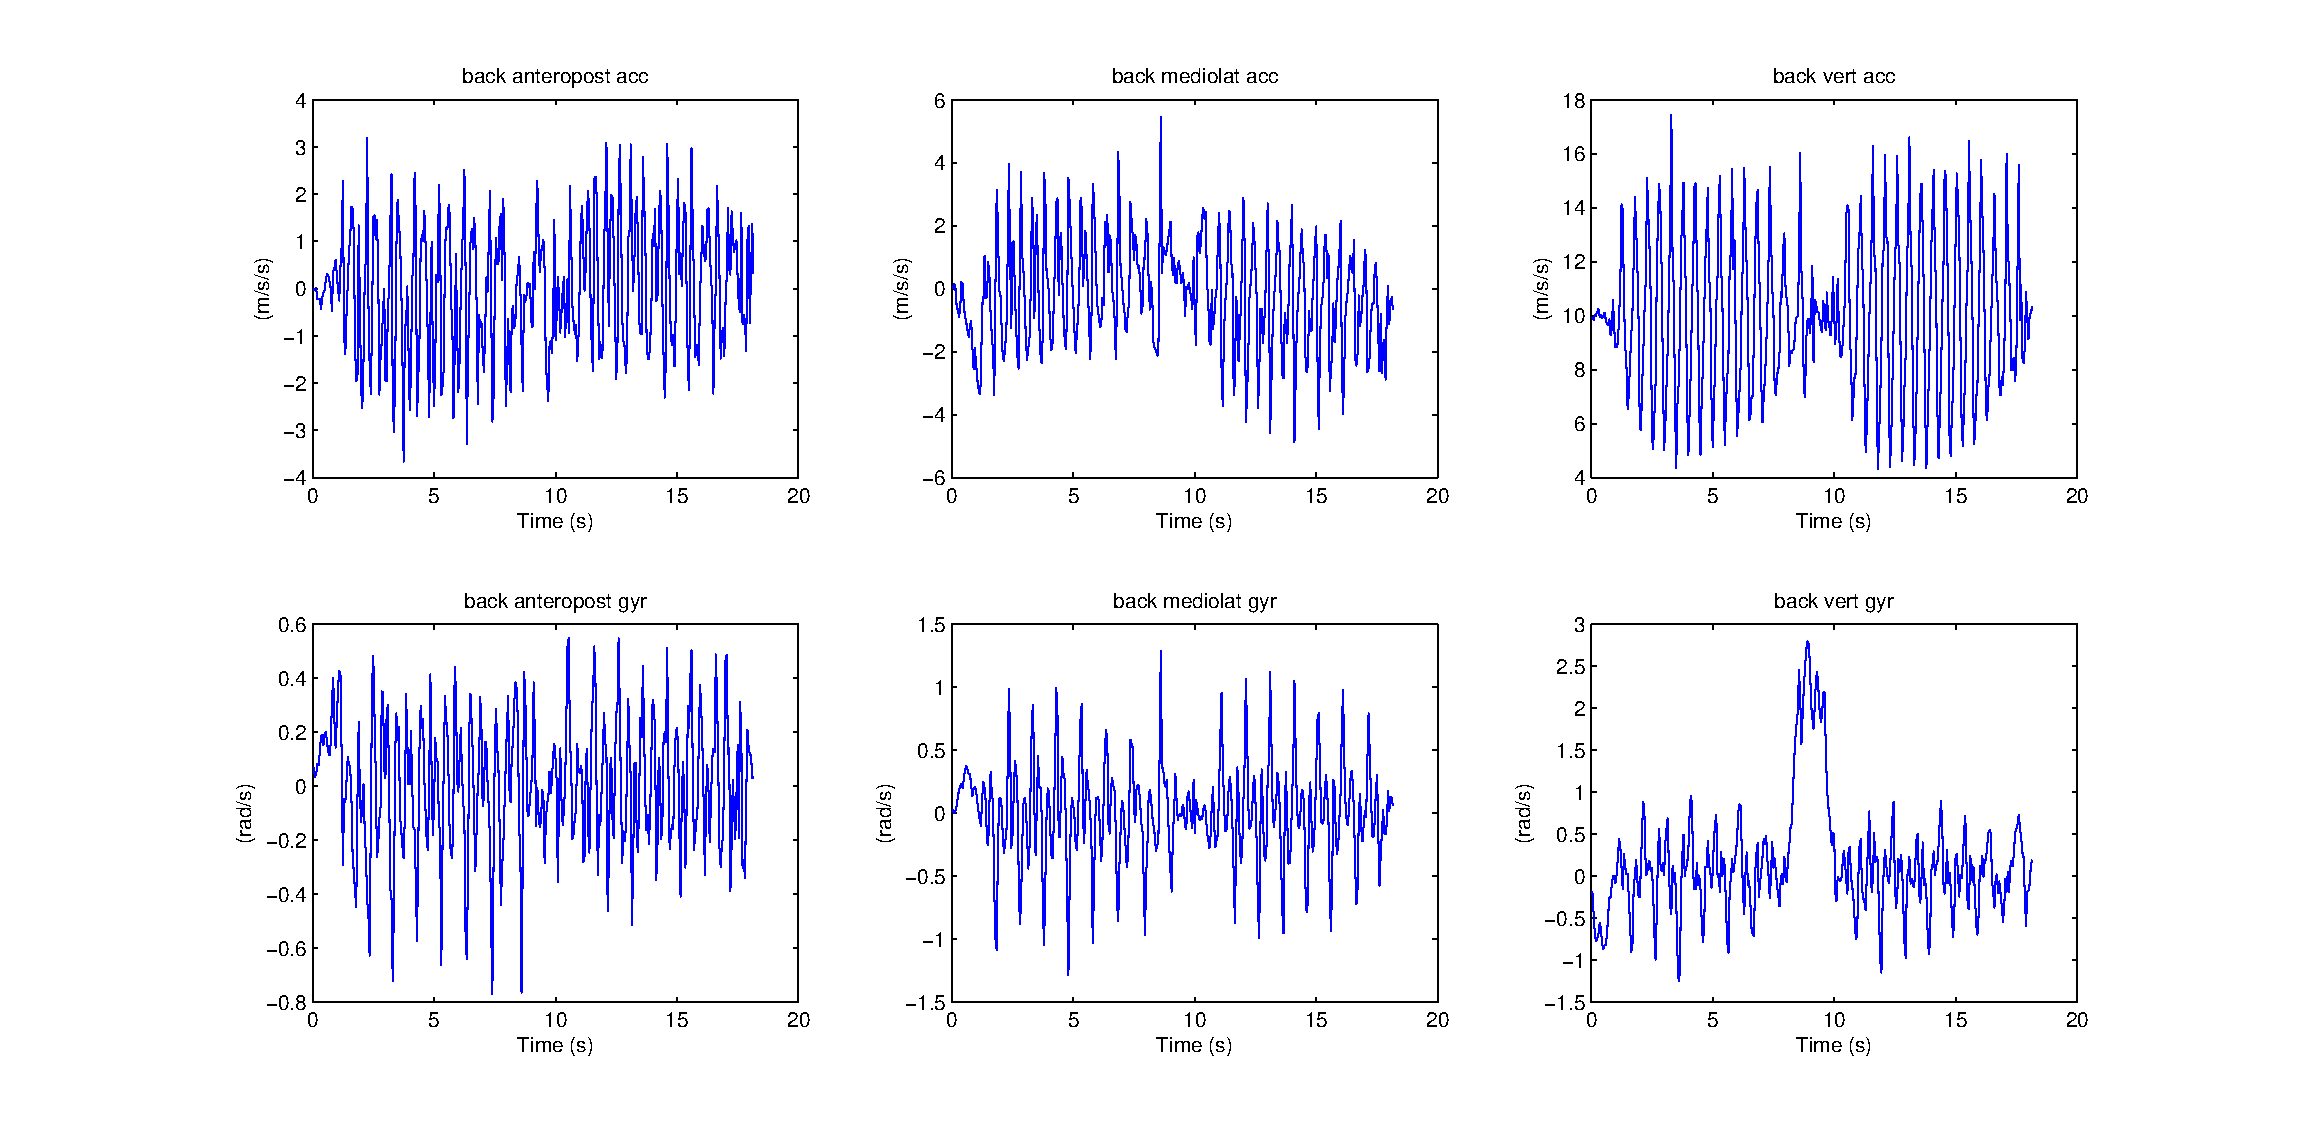
\includegraphics[scale=0.4]{examplevisuback}

\end{frame}

\begin{frame}
\frametitle{Example of foot IMU record}
\hspace*{-2.8cm}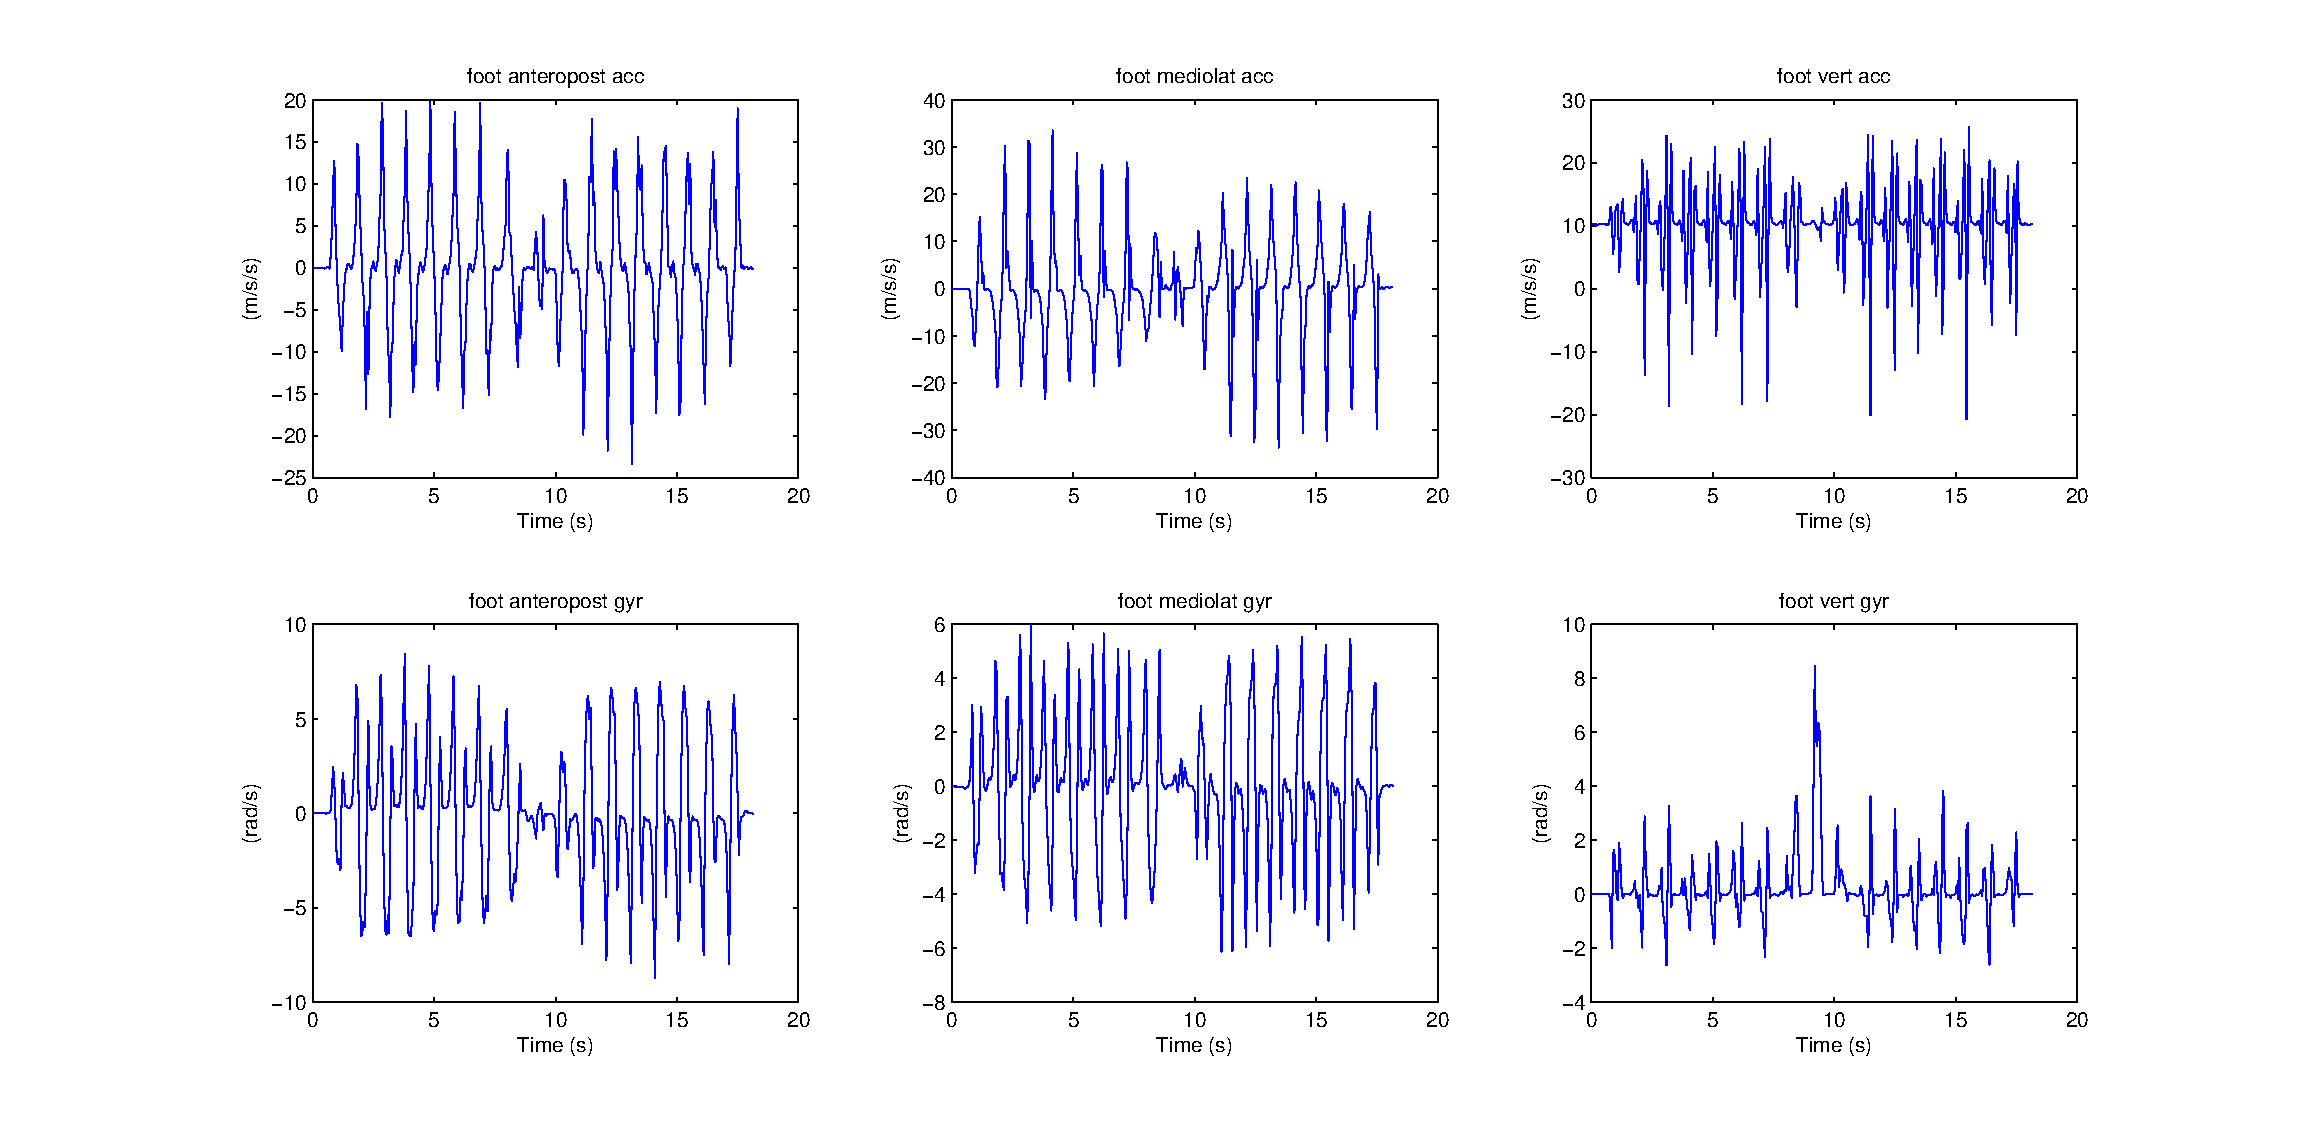
\includegraphics[scale=0.4]{examplevisufoot}

\end{frame}

\section{Windowed approach}
\subsection{With Fourier}

\begin{frame}
\begin{itemize}
\item[Ref.] \emph{Classification of periodic activities using the Wasserstein distance}, L. Oudre, J. Jakubowicz, P. Bianchi, C. Simon

\item[Frequency] spectrum bandwidthed from 0.5 to 5 Hz on a window

\item[Wasserstein] distance is less shift-sensitive, used in image and music signal processing
\[d_W(g,h)=\int_0^\pi\left|\int_0^xg(t)-h(t)dt\right|dx\]

\item[Point]to point distance
\[d(x,y)=d_W(\frac x{||x||_1},\frac y{||y||_1})+\mu\cdot\left|\phantom{\frac{}{}}||x||_1-||y||_1\right|\]
\end{itemize}
\end{frame}

\begin{frame}
\frametitle{Application back angular velocities :\\16 and 32-sampled windows, 75\% overlap}
\hspace*{-1.8cm}\includegraphics[scale=0.47]{examplewasser16gyr}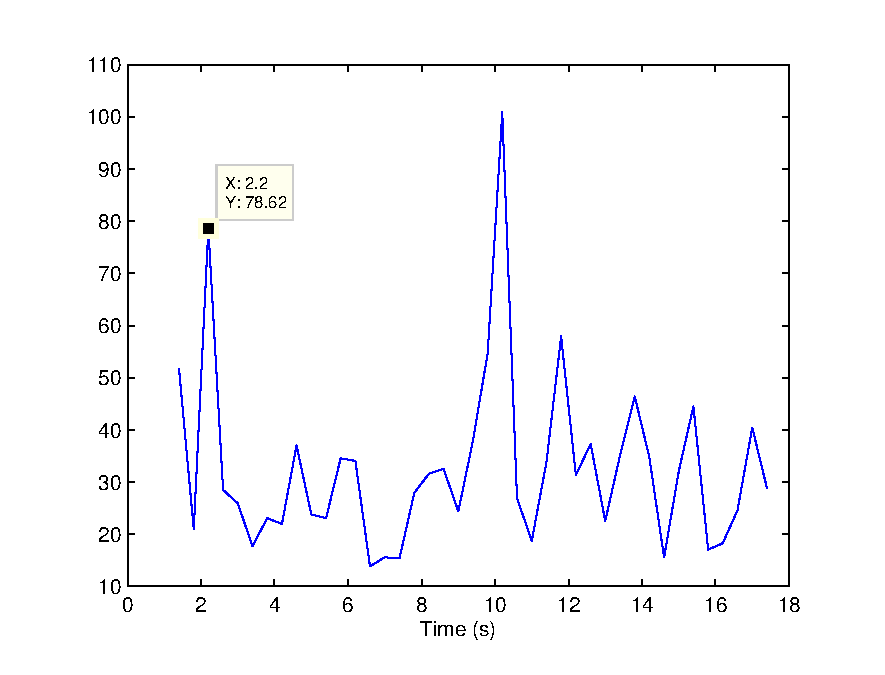
\includegraphics[scale=0.47]{examplewasser32gyr}
\end{frame}

\subsection{With statistics}
\begin{frame}
\begin{itemize}
\item[Many] proposed features in literature :
\item $a_{ML}+a_V$, $a_{AP}$ and $a_V$ means ;
\item $a_{AP}+a_V$ and $a_{ML}$ standard-deviations ;
\item $a_V$ median;
\item $a_{ML}$ 95-percentile; \emph{etc}

\item[Good] results with kurtosis
\item[Issue] on window length : accuracy/smooth trade-off, hard under 100 Hz
\end{itemize}
\end{frame}

\begin{frame}
\hspace*{-2cm}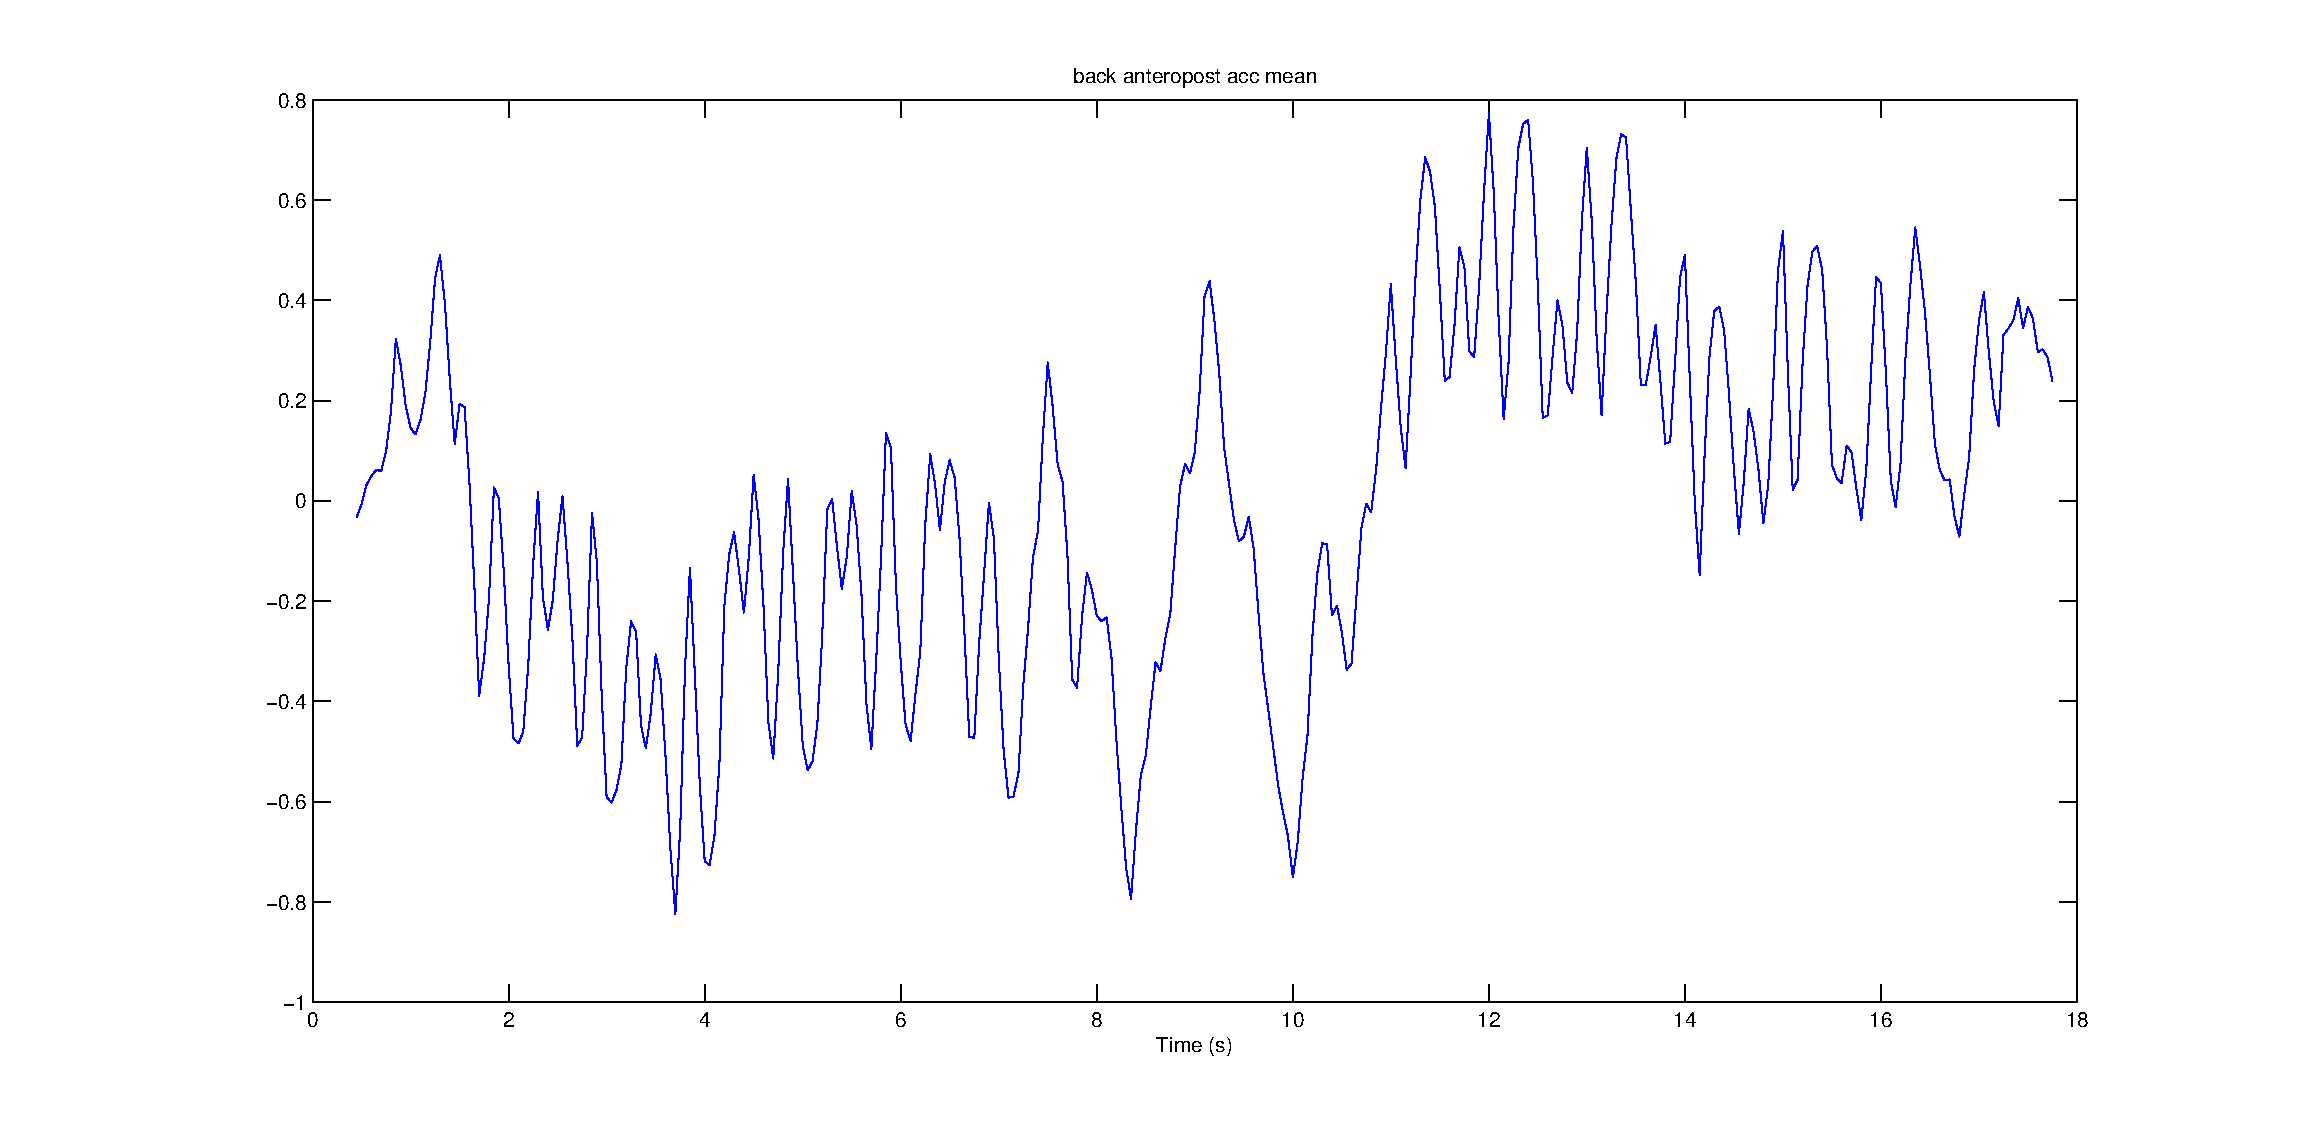
\includegraphics[height=4.4cm,width=6.9cm]{examplew16moyAap}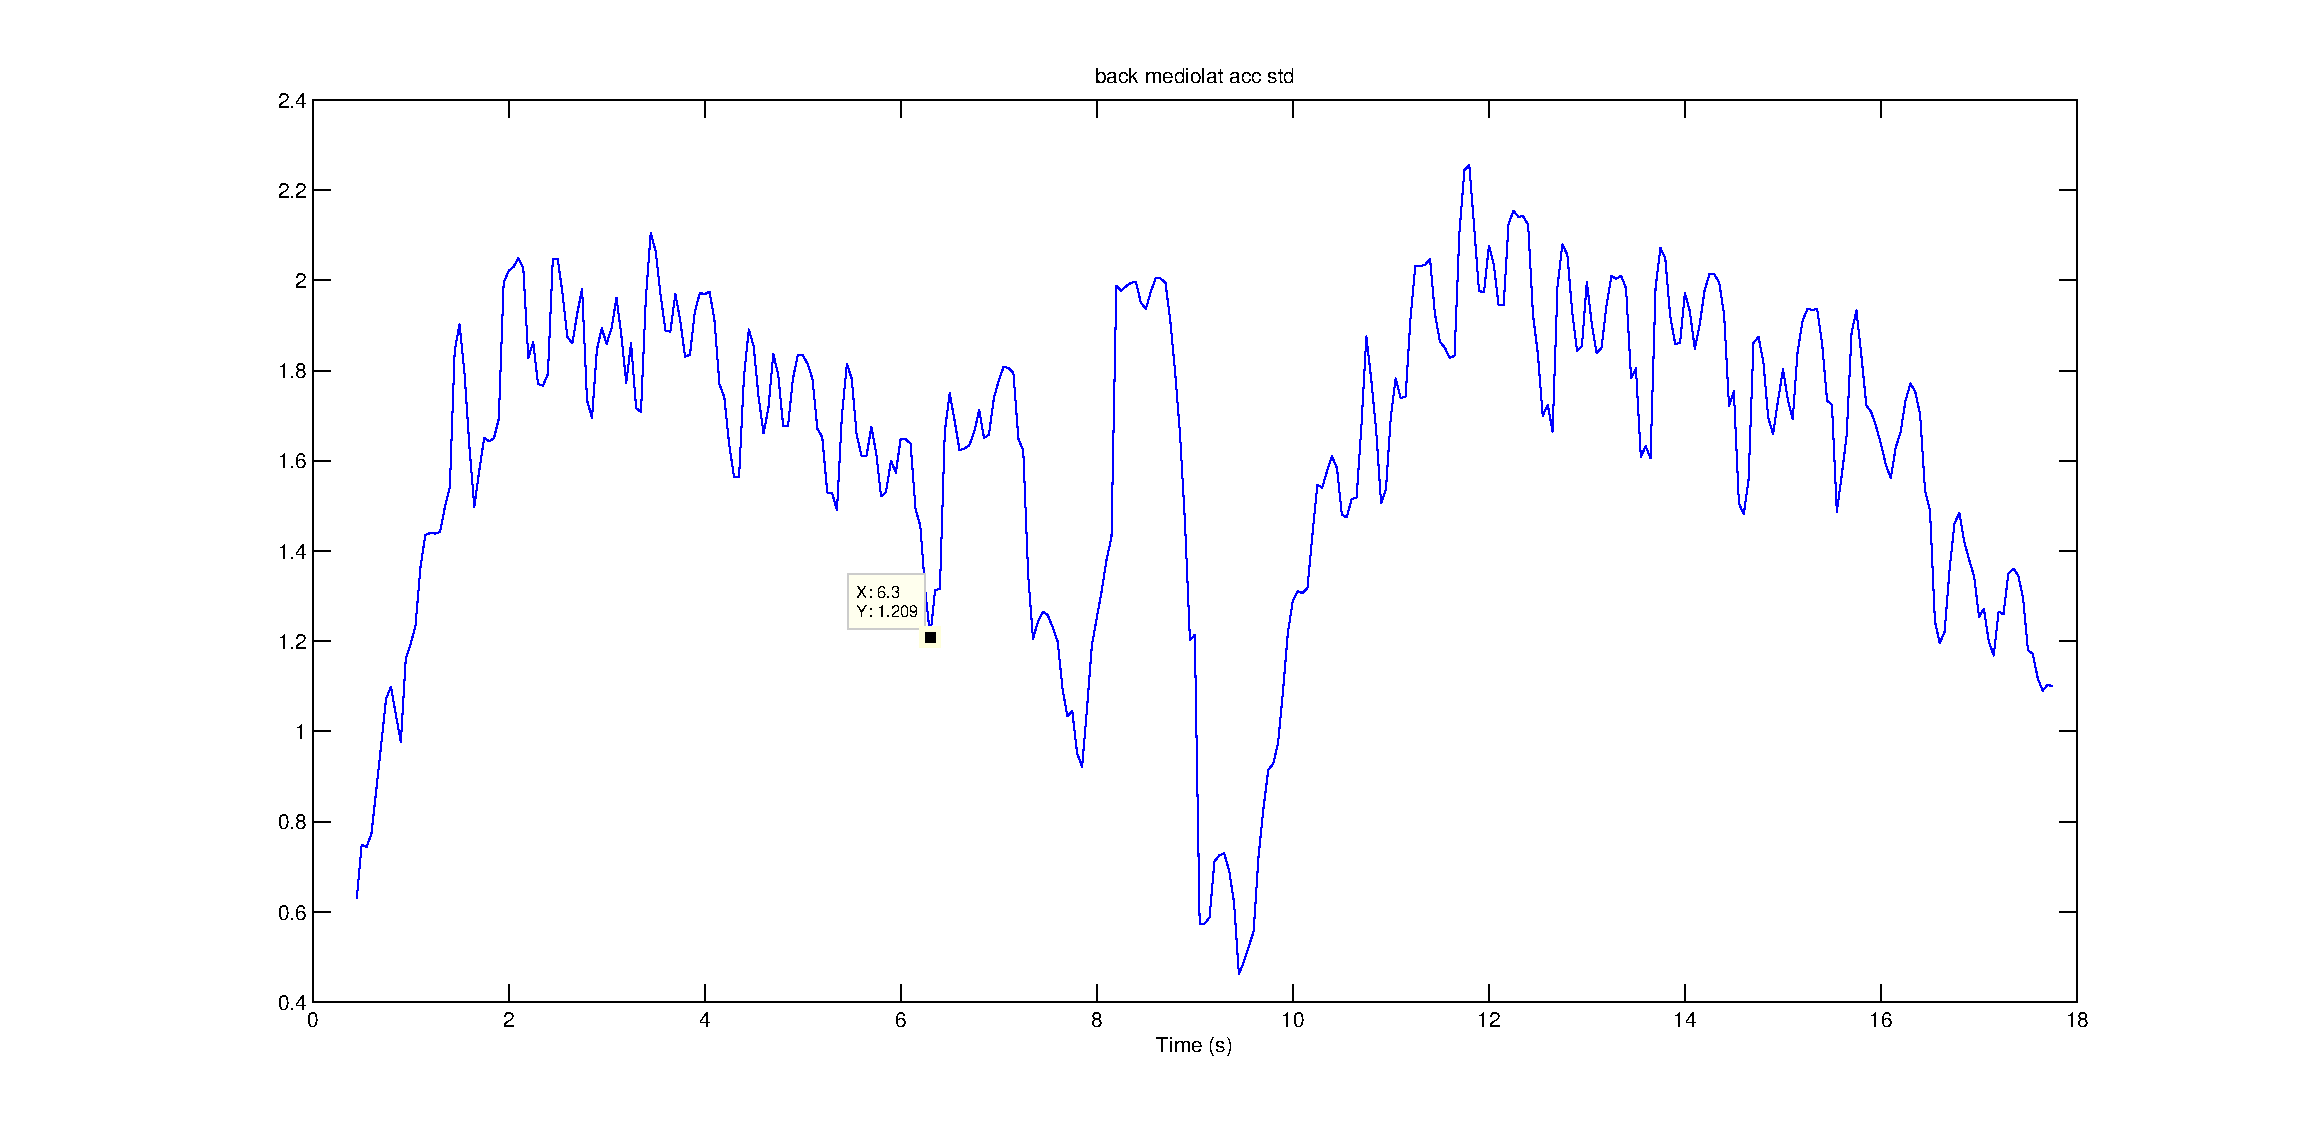
\includegraphics[height=4.4cm,width=6.9cm]{examplew16stdAml}
\\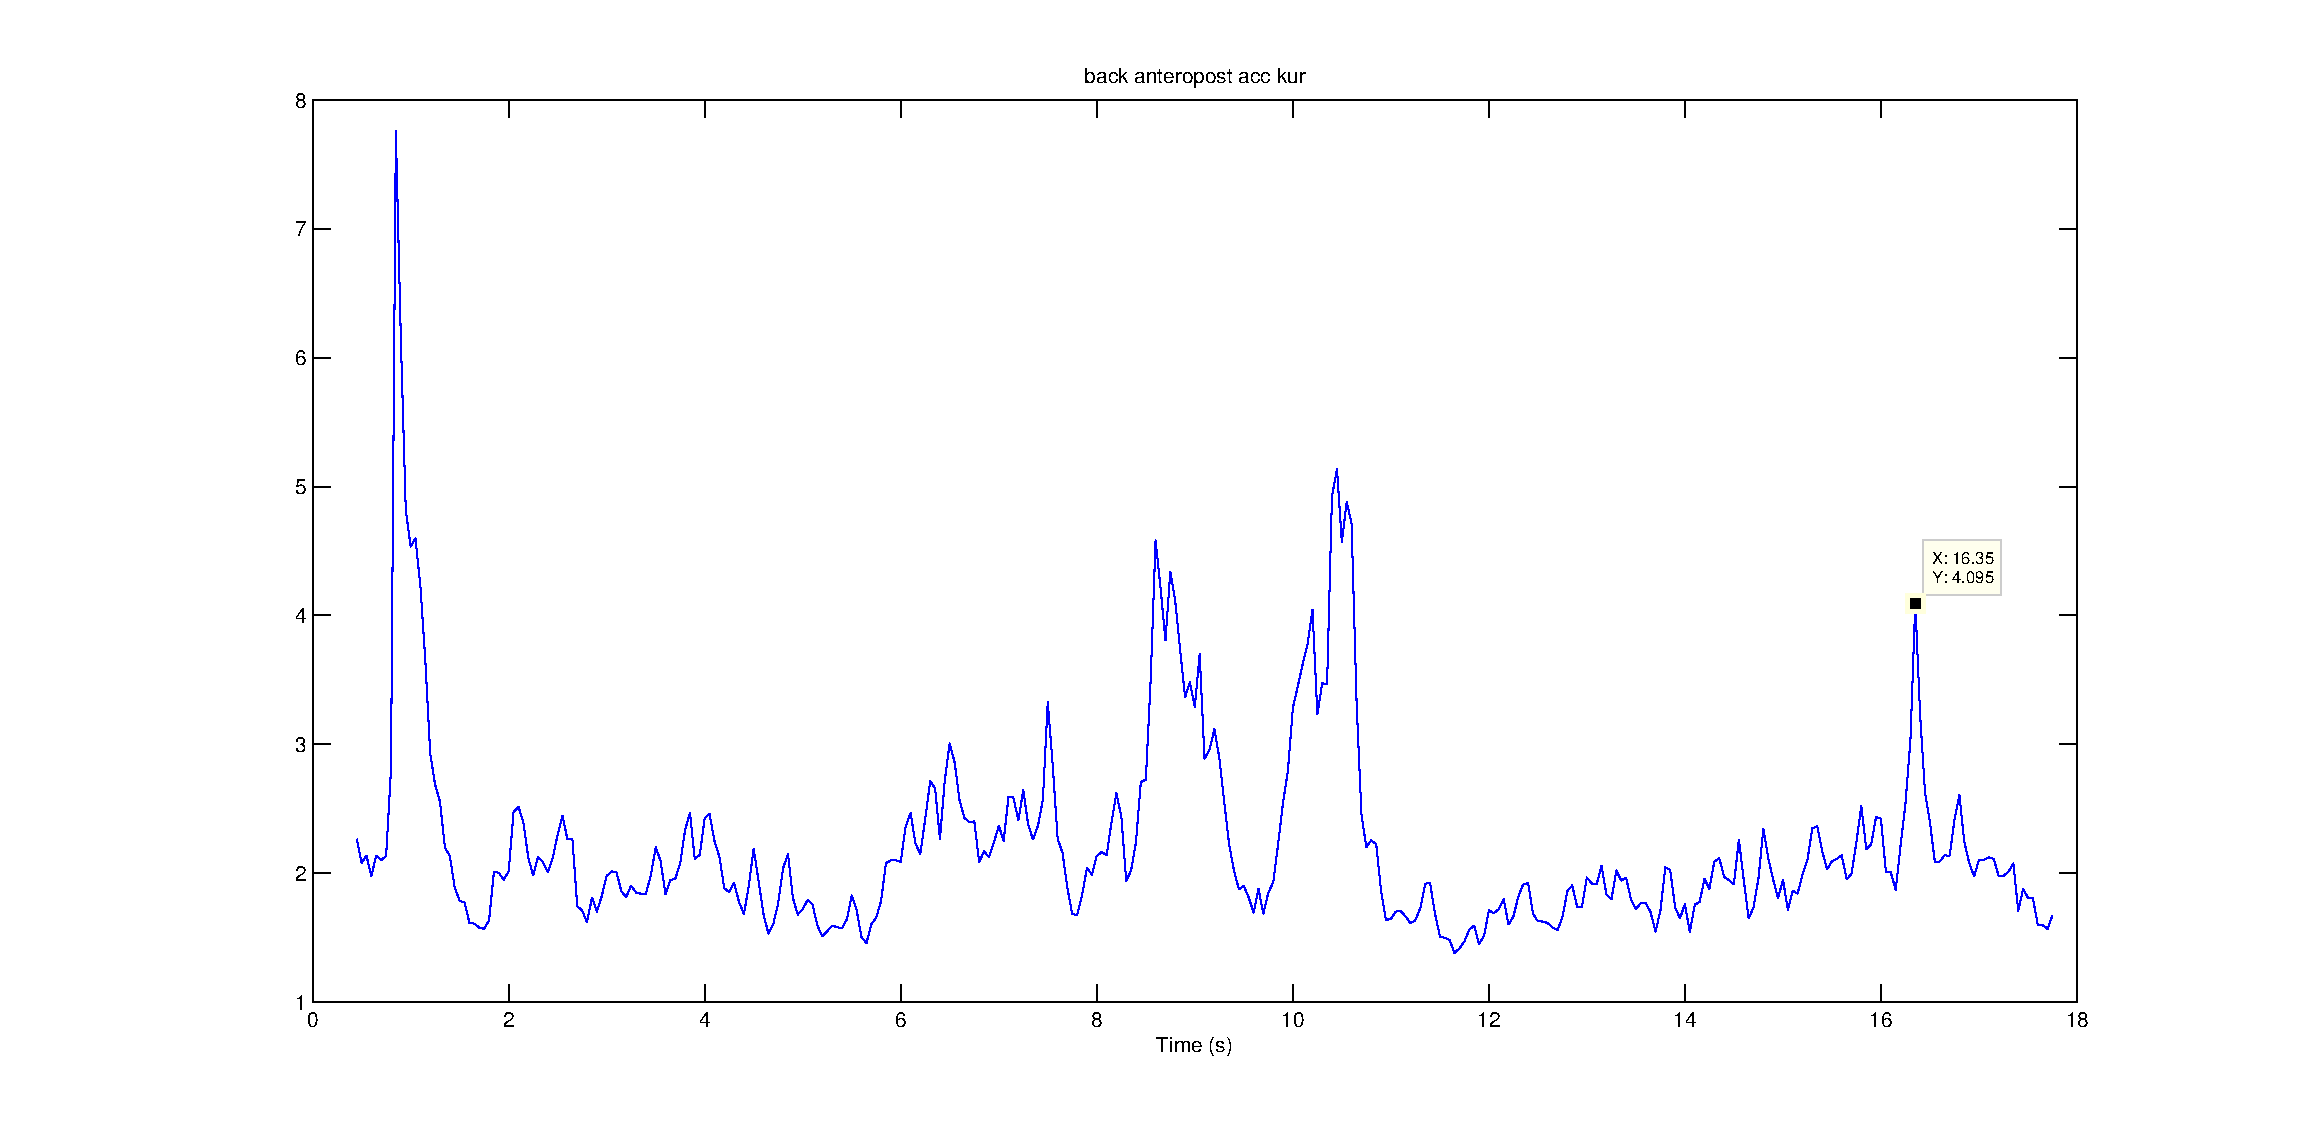
\includegraphics[height=4.4cm]{examplew16kurAap}
\end{frame}

\section{CUSUM algorithm}
\subsection{Working}

\begin{frame}
\begin{itemize}
\item[Ref.] \emph{Detection of Abrupt Changes : Theory and Application},\\
M. Basseville, I. V. Nikiforov (1993)
\item[Proposed] by E. S. Page in 1954
\item[Based] on maxima of likelihood estimated
\[\tilde\varLambda_1^N(k)=\inf_{\tilde\theta_0}\sup_{\theta_0}\sup_{\theta_1}\ln\left[\frac{\prod_{i=1}^{k-1}p_{\theta_0}(y_i)\cdot\prod_{i=k}^Np_{\theta_0}(y_i)}{\prod_{i=1}^Np_{\tilde\theta_0}(y_i)}\right]\]
\[\hat t_0=\arg\max_{1\le k\le N}\tilde\varLambda_1^N(k)\]
\item[Assume] independent signals under normal distribution
\item[Applied] on acceleration norms and yaw by dichotomy
\end{itemize}
\end{frame}

\subsection{First results}

\begin{frame}
\hspace*{-2.8cm}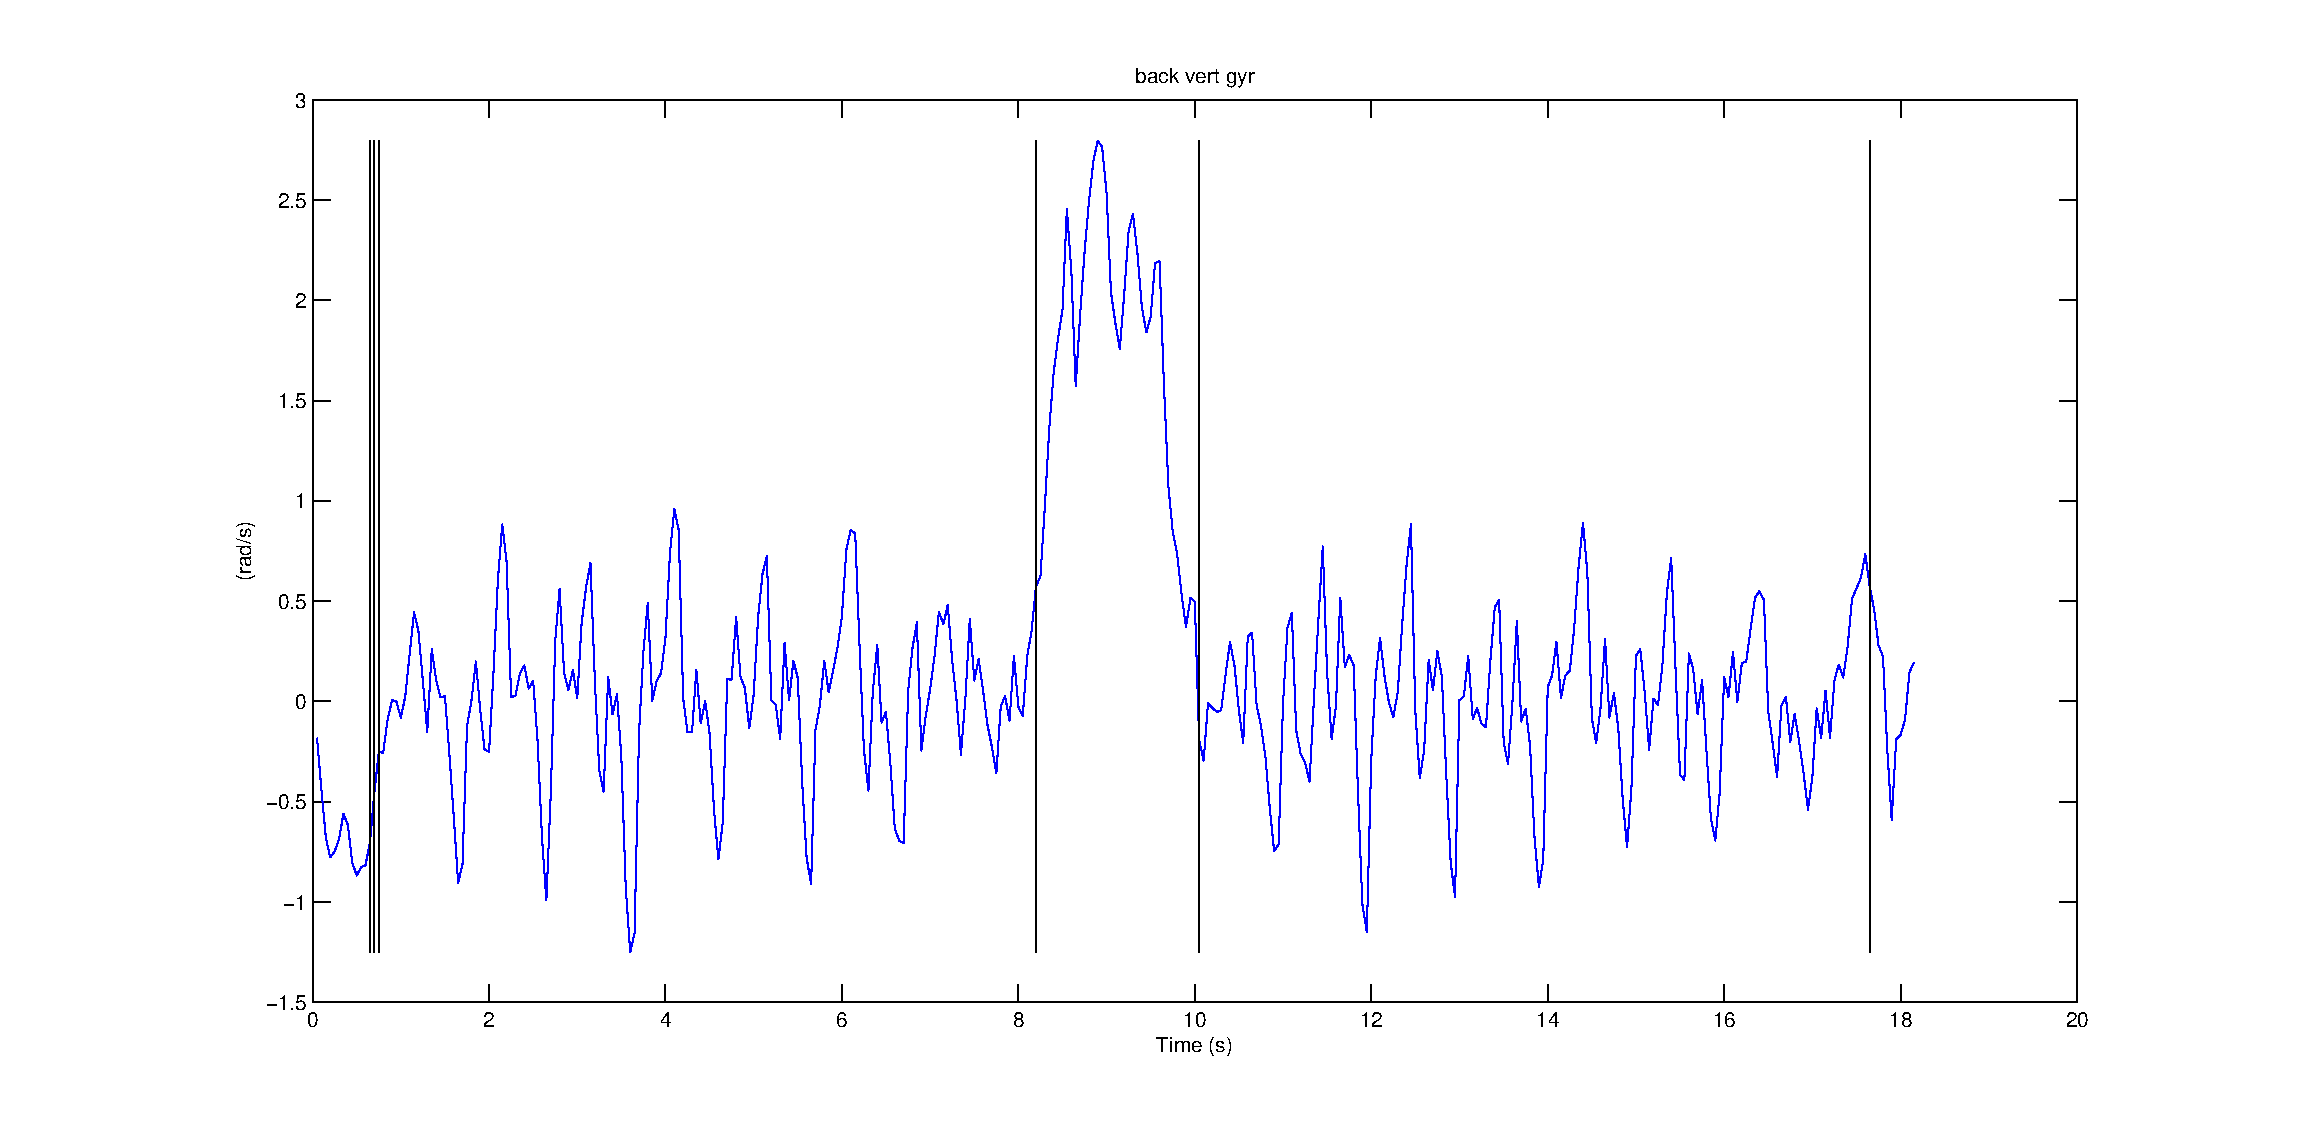
\includegraphics[scale=0.4]{examplecusumbackvertgyr}
\end{frame}

\end{document}